\documentclass[]{article}
\makeatletter\if@twocolumn\PassOptionsToPackage{switch}{lineno}\else\fi\makeatother

%Publisher: Emerald Publishing
%Template Provided By: Typeset

\usepackage{amsmath,tabulary,graphicx,times,caption,fancyhdr,amssymb,amsfonts,amstext,amsbsy}
\usepackage[utf8]{inputenc}
\usepackage[T1]{fontenc}
\usepackage[paperheight=10in,paperwidth=6.5in,margin=2cm,headsep=.5cm,headheight=1.5cm,top=2.5cm]{geometry}
\renewenvironment{abstract} {\vspace*{-1pc}\trivlist\item[]\leftskip\oupIndent\hrulefill\par\vskip4pt\noindent\textbf{\abstractname}\mbox{\null}\\}{\par\noindent\hrulefill\endtrivlist} 
\linespread{1.13} \date{}
\captionsetup[figure]{labelfont=sc,skip=1.4pt,aboveskip=1pc}
\captionsetup[table]{labelfont=sc,skip=1.4pt,labelsep=newline}

%%%%%%%%%%%%%%%%%%%%%%%%%%%%%%%%%%%%%%%%%%%%%%%%%%%%%%%%%%%%%%%%%%%%%%%%%%
% Following additional macros are required to function some 
% functions which are not available in the class used.
%%%%%%%%%%%%%%%%%%%%%%%%%%%%%%%%%%%%%%%%%%%%%%%%%%%%%%%%%%%%%%%%%%%%%%%%%%
\usepackage{url,multirow,morefloats,floatflt,cancel,tfrupee}
\makeatletter


\AtBeginDocument{\@ifpackageloaded{textcomp}{}{\usepackage{textcomp}}}
\makeatother
\usepackage{colortbl}
\usepackage{xcolor}
\usepackage{pifont}
\usepackage{longtable}  % For long tables spanning multiple pages
\usepackage{booktabs}   % For top, mid and bottom rules
\usepackage{caption}  % For captions in floating environments
\usepackage{array}      % For table column formatting
\usepackage{geometry}   % Optional: For setting page margins
\usepackage{pdflscape}  % For the landscape environment
\usepackage{microtype}
\usepackage{float}
\usepackage[nointegrals]{wasysym}
\urlstyle{rm}
\makeatletter

%%%For Table column width calculation.
\def\mcWidth#1{\csname TY@F#1\endcsname+\tabcolsep}

%%Hacking center and right align for table
\def\cAlignHack{\rightskip\@flushglue\leftskip\@flushglue\parindent\z@\parfillskip\z@skip}
\def\rAlignHack{\rightskip\z@skip\leftskip\@flushglue \parindent\z@\parfillskip\z@skip}

%Etal definition in references
\@ifundefined{etal}{\def\etal{\textit{et~al}}}{}


%\if@twocolumn\usepackage{dblfloatfix}\fi
\usepackage{ifxetex}
\ifxetex\else\if@twocolumn\@ifpackageloaded{stfloats}{}{\usepackage{dblfloatfix}}\fi\fi

\AtBeginDocument{
\expandafter\ifx\csname eqalign\endcsname\relax
\def\eqalign#1{\null\vcenter{\def\\{\cr}\openup\jot\m@th
  \ialign{\strut$\displaystyle{##}$\hfil&$\displaystyle{{}##}$\hfil
      \crcr#1\crcr}}\,}
\fi
}

%For fixing hardfail when unicode letters appear inside table with endfloat
\AtBeginDocument{%
  \@ifpackageloaded{endfloat}%
   {\renewcommand\efloat@iwrite[1]{\immediate\expandafter\protected@write\csname efloat@post#1\endcsname{}}}{\newif\ifefloat@tables}%
}%

\def\BreakURLText#1{\@tfor\brk@tempa:=#1\do{\brk@tempa\hskip0pt}}
\let\lt=<
\let\gt=>
\def\processVert{\ifmmode|\else\textbar\fi}
\let\processvert\processVert

\@ifundefined{subparagraph}{
\def\subparagraph{\@startsection{paragraph}{5}{2\parindent}{0ex plus 0.1ex minus 0.1ex}%
{0ex}{\normalfont\small\itshape}}%
}{}

% These are now gobbled, so won't appear in the PDF.
\newcommand\role[1]{\unskip}
\newcommand\aucollab[1]{\unskip}
  
\@ifundefined{tsGraphicsScaleX}{\gdef\tsGraphicsScaleX{1}}{}
\@ifundefined{tsGraphicsScaleY}{\gdef\tsGraphicsScaleY{.9}}{}
% To automatically resize figures to fit inside the text area
\def\checkGraphicsWidth{\ifdim\Gin@nat@width>\linewidth
	\tsGraphicsScaleX\linewidth\else\Gin@nat@width\fi}

\def\checkGraphicsHeight{\ifdim\Gin@nat@height>.9\textheight
	\tsGraphicsScaleY\textheight\else\Gin@nat@height\fi}

\def\fixFloatSize#1{}%\@ifundefined{processdelayedfloats}{\setbox0=\hbox{\includegraphics{#1}}\ifnum\wd0<\columnwidth\relax\renewenvironment{figure*}{\begin{figure}}{\end{figure}}\fi}{}}
\let\ts@includegraphics\includegraphics

\def\inlinegraphic[#1]#2{{\edef\@tempa{#1}\edef\baseline@shift{\ifx\@tempa\@empty0\else#1\fi}\edef\tempZ{\the\numexpr(\numexpr(\baseline@shift*\f@size/100))}\protect\raisebox{\tempZ pt}{\ts@includegraphics{#2}}}}

%\renewcommand{\includegraphics}[1]{\ts@includegraphics[width=\checkGraphicsWidth]{#1}}
\AtBeginDocument{\def\includegraphics{\@ifnextchar[{\ts@includegraphics}{\ts@includegraphics[width=\checkGraphicsWidth,height=\checkGraphicsHeight,keepaspectratio]}}}

\DeclareMathAlphabet{\mathpzc}{OT1}{pzc}{m}{it}

\def\URL#1#2{\@ifundefined{href}{#2}{\href{#1}{#2}}}

%%For url break
\def\UrlOrds{\do\*\do\-\do\~\do\'\do\"\do\-}%
\g@addto@macro{\UrlBreaks}{\UrlOrds}



\edef\fntEncoding{\f@encoding}
\def\EUoneEnc{EU1}
\makeatother
\def\floatpagefraction{0.8} 
\def\dblfloatpagefraction{0.8}
\def\style#1#2{#2}
\def\xxxguillemotleft{\fontencoding{T1}\selectfont\guillemotleft}
\def\xxxguillemotright{\fontencoding{T1}\selectfont\guillemotright}

\newif\ifmultipleabstract\multipleabstractfalse%
\newenvironment{typesetAbstractGroup}{}{}%

%%%%%%%%%%%%%%%%%%%%%%%%%%%%%%%%%%%%%%%%%%%%%%%%%%%%%%%%%%%%%%%%%%%%%%%%%%





\usepackage[noindentafter]{titlesec}
\def\NormalBaseline{\def\baselinestretch{1.1}}

\titleformat{\section}[hang]{\NormalBaseline\filright\large\fontsize{12}{15}\bfseries\boldmath}
{\large\thesection.}
{10pt}
{\noindent}
[]
\titleformat{\subsection}[hang]{\NormalBaseline\filright\fontsize{11}{13}\bfseries\itshape\boldmath}
{\thesubsection.}
{10pt}
{}
[]
\titleformat{\subsubsection}[hang]{\NormalBaseline\filright\fontsize{10}{12}\bfseries\itshape\boldmath}
{\thesubsubsection.}
{10pt}
{}
[]
\titleformat{\paragraph}[runin]{\NormalBaseline\filright\itshape}
{\theparagraph.}
{10pt}
{}
[]
\titleformat{\subparagraph}[runin]{\NormalBaseline\filright\itshape}
{\thesubparagraph.}
{10pt}
{}
[]


\titlespacing{\section}{0pt}{1.5\baselineskip}{.2\baselineskip}  
\titlespacing{\subsection}{0pt}{1\baselineskip}{.2\baselineskip}  
\titlespacing{\subsubsection}{0pt}{1.5\baselineskip}{.2\baselineskip}  
\titlespacing{\paragraph}{0pt}{.5\baselineskip}{10pt}  
\titlespacing{\subparagraph}{0pt}{.5\baselineskip}{10pt}  



\makeatletter\def\oupIndent{1pt}
\def\author#1{\gdef\@author{\hskip-\dimexpr(\tabcolsep)\hskip\oupIndent\parbox{\dimexpr\textwidth-\oupIndent}{\centering\bfseries#1}}}
\def\title#1{\gdef\@title{\centering\bfseries\ifx\@articleType\@empty\else\@articleType\\\fi#1}}
\let\@articleType\@empty \def\articletype#1{\gdef\@articleType{{\normalfont\itshape#1}}}
\fancypagestyle{headings}{\fancyhf{}\fancyhead[C]{\RunningHead\hspace*{1pc}}\fancyhead[R]{\thepage}}\pagestyle{headings}
\emergencystretch =15pt 
\makeatother
\usepackage[authoryear, round]{natbib} % authoryear for author-year citations, round for parentheses
\usepackage[hidelinks]{hyperref}

\begin{document}


\title{JIT, Environmental Practices \& Performance: an empirical analysis}
\author{Alessa Aila\textsuperscript{1}\thanks{E-mail: alessa.aila@aalto.fi}{ },
            Astrid Holmstr{\"{o}}m\textsuperscript{1}\thanks{E-mail: astrid.holmstrom@aalto.fi}{ },
            Eemil Rantala\textsuperscript{1}\thanks{E-mail: eemil.rantala@aalto.fi}{ },
            John Anderson\textsuperscript{1}\thanks{E-mail: john.anderson@aalto.fi}{ } and
            Valtteri Luodem{\"{a}}ki\textsuperscript{1}\thanks{E-mail: valtteri.luodemaki@aalto.fi}{ }~\\[-3pt]\normalsize\normalfont\itshape 
~\\\textsuperscript{1}{Department of Industrial Engineering and Management\unskip, Aalto University}}
\def\RunningHead{{JIT, Environmental Practices \& Performance: an empirical analysis}}

\maketitle 


\begin{abstract}
\textbf{Purpose} - This paper aims to identify if there are complimentarity effects on environmental sustainability produced from JIT \& environmental practices. 
Due to the increased delivery frequency and pacakging requirements implied by JIT we also investigate the moderating effect between JIT and environmental practices on air emissions and solid waste generation. 
\\
\textbf{Design/methodology/approach} - This paper uses the High Performance Manufacturing dataset (Round IV). This survey includes plants across 19 countries across Europe, Asia and the Americas.
The industries included in the study are machinery, electronics and transportation.
\\
\textbf{Findings} - Our results suggest that there is no complimentarity effect between JIT and environmental practices on environmental performance. Our study also finds no moderating effect between JIT and environmental practices on air emissions and solid waste generation.
\\
\textbf{Research limitations/ implications} - We suggest more work to be done on the analysis, specifically on the robustness checks and the control variables used in the regression analysis.
\end{abstract}\def\keywordstitle{Keywords}
\section{Introduction}
Over the past decade there has been an increase in the research published on the synergies and trade-offs between lean manufacturing and environmental performance \citep{henaoLeanManufacturingSustainable2019, abualfaraaLeanGreenManufacturingPractices2020, diesteRelationshipLeanEnvironmental2019, lobomesquitaExploringRelationshipsIntegrating2022, garza-reyesLeanGreenSystematic2015, kingLeanGreenEmpirical2009}.

These combined approaches, often dubbed `lean-green', typically cites the Triple-Bottom-Line concept, which postulates the need for performance in economic growth, environmental preservation, and social responsibility, in order to achieve sustainability \citep{henaoLeanManufacturingSustainable2019}. 
Motivated by this body of research as well as our interest in sustainability studies, we have decided to study the effect of environmental and lean practices on environmental performance. 

Abualfaraa et al. outline several research gaps and opportunities for those interested in lean-green manufacturing. 
In their Structured Literature Review of articles published between 2000 and 2018, they have identified several research directions in both the synergies and incompatibilities between environmental and lean practices \citep{abualfaraaLeanGreenManufacturingPractices2020}. 
On one line, it is argued that lean practices may work as a catalyst for environmental practices and innovation through its focus on waste reduction and continuous improvement.
On the other, the incompatibilities between the two approaches are also studied. 
Just in time (JIT) practices have been specifically highlighted. 
For example JIT manufacturing practices such as small lot sizes and high replenishment frequency implies more frequent transportation, higher CO2 emissions and more packaging waste \citep{diesteRelationshipLeanEnvironmental2019}.

Literature reviews also pointed out the need for more quantitative research with a focus on robust, well-defined sustainability metrics \citep{abualfaraaLeanGreenManufacturingPractices2020}. 
Through an empirical analysis of JIT and environmental practices, our goal is to contribute to this research agenda.
\section{Environmental Practices}
A key concept in our research is environmental practices. 
In academic literature, ‘environmental practices’ is used to describe a wide range of different environmental practices \citep{montabonExaminationCorporateReporting2007}. 
However, environmental practices are highly context-related and in our paper we will focus specifically on environmental practices in a manufacturing plant context. 
There are a lot of environmental practices present in the literature and generating an exhaustive list would be impossible. 
Separating environmental practices from non-environmental practices is not simple as many conventional practices can be perceived as environmental practices depending on the context.

There are also various other terms and concepts that are closely related to environmental practices depending on the context. 
Many articles include discussion about environmental management practices which can be seen as environmental practices. 
The term ‘green practices’ is also occasionally mentioned and it is often interchangeable with the concept of environmental practices.

For the purpose of examining environmental practices, researchers have developed multiple sets of environmental practices that are used in the papers for analysis and surveys \citep{montabonExaminationCorporateReporting2007, zhuRelationshipsOperationalPractices2004}. 
In the literature, different categorizations for environmental practices have been displayed. 
Montabon et al. (2007) divided their list of environmental practices used in their study into operational, tactical and strategic practices. 
This was done in order to recognize that different practices have different scopes and impacts \citep{montabonExaminationCorporateReporting2007}. 
In our research, we will consider environmental practices comprehensively and use a list of environmental practices developed by the HPM survey.
\section{Lean practices and JIT delivery}
\subsection{Lean as a concept}
Lean manufacturing refers to manufacturing where lean has been implemented. 
There are a lot of different definitions for lean in academic literature \citep{sundarReviewLeanManufacturing2014}. 
Lean is often thought of as activities relating to waste reduction, but in practice the fundamental purpose of lean is to increase the value of output by reducing waste in production processes \citep{sundarReviewLeanManufacturing2014}. 
For this paper, lean is defined loosely as a system that aims at continuous improvement and elimination of all kinds of waste \citep{simpsonUseSupplyRelationship2005}. 
Lean practices include for example Just-in-Time manufacturing, Kanban, value stream mapping, and push and pull systems \citep{sundarReviewLeanManufacturing2014}. 
The main benefits of lean relate to increased productivity and quality while costs are reduced \citep{bhamuLeanManufacturingLiterature2014}.

Lean manufacturing is a holistic way of working. 
\citep{kingLeanGreenEmpirical2009} point out that lean manufacturing includes numerous practices, which spread over the entire scope of the organisation. 
Lean manufacturing can thus be seen to cover aspects of product development, operations management, supply chain management, design and manufacturing \citep{bhamuLeanManufacturingLiterature2014}. 
\citep{sundarReviewLeanManufacturing2014} add that lean implementation requires a proper sequencing and integration plan. 
For example, cultural change and employee training on lean concepts are needed to make the implementation successful.

\subsection{Just-in-time delivery}
In the literature, the concepts of lean and Just-In-Time are intertwined and many, such as \citep{bhamuLeanManufacturingLiterature2014}, \citep{belekoukiasImpactLeanMethods2014} recognize the close connection between them. 
Just-in-Time is a critical aspect of lean manufacturing practices, focusing on the efficiency of production timing and inventory management.

“Lean manufacturing has been widely implemented by manufacturing organisations to achieve operational excellence, and in this way meet both traditional and contemporary organisational objectives such as profitability, efficiency, responsiveness, quality and customer satisfaction” \citep{garza-reyesLeanGreenSystematic2015}. 
“JIT is based on producing the right goods at the right time” \citep{womackLeanThinkingBanish1997}. 
This contributes in reducing space utilisation, inventory and wastes associated to the overproduction of goods.

\section{Environmental performance}
Environmental performance means how well an organisation performs in relation to its environmental responsibilities \citep{mollenkopfGreenLeanGlobal2010}. 
It is measured by how much natural resources have been consumed and by how much waste of water, gases and poisonous materials are emitted \citep{maoLowCarbonSupply2017}. 
In this paper, the focus is on studying the environmental performance of manufacturing plants. 
We do not consider how the manufacturing plant contributes to the environmental performance of the whole supply chain. 

% Subsections for CO2 emissions and Packaging waste

\section{Relationship between JIT and environmental performance}
Most of the existing literature states that lean practices used to decrease the environmental impact of a company are successful \citep{diesteEvaluatingImpactLean2020}. 
However, there are different opinions among scholars on whether lean practices have a positive impact on environmental performance and lean practices can according to the literature have both positive and negative impacts on environmental performance \citep{diesteEvaluatingImpactLean2020}.

According to the research conducted by \citep{diesteEvaluatingImpactLean2020}, the general trend seems to be that lean practices improve long term environmental performance. 
Lean processes can aid companies in achieving their environmental goals if they are committed to the goals and aware of the organisation’s environmental impact \citep{diesteEvaluatingImpactLean2020}. 
Some researchers state that lean companies can improve their environmental performance since the lean practices also focus on waste reduction and process efficiency \citep{diesteEvaluatingImpactLean2020}. 
More specifically, JIT practices can improve the environmental supply chain performance \citep{cherrafiLeanGreenPractices2018, diesteEvaluatingImpactLean2020} and decrease the fuel consumption since smaller vehicles can be used for smaller deliveries \citep{garza-reyesLeanGreenTransport2016}. 
Further, JIT can reduce energy consumption of storage since it reduces the inventory volume \citep{garza-reyesEffectLeanMethods2018}.

Additionally, since lean practices assert waste reduction, they can naturally lead to better environmental practices and an internal environment that supports the adaptation of these practices \citep{garza-reyesEffectLeanMethods2018}. 
Further, aspects worth considering are that lean companies more likely adapt environmental innovations \citep{mollenkopfGreenLeanGlobal2010, garza-reyesEffectLeanMethods2018}. 

However, being more productive and efficient in manufacturing does not equal more environmental sustainability and several papers address negative or mixed impacts of lean on air emissions, energy use and water use \citep{diesteEvaluatingImpactLean2020}. 
Out of the lean practices, JIT is the most problematic due to its nature of small deliveries which can increase additional waste and emissions \citep{rothenbergLEANGREENQUEST2009, Venkat_Wakeland_2006, diesteEvaluatingImpactLean2020} and some scholars argue that JIT and positive environmental performance cannot be combined \citep{zhuRelationshipsOperationalPractices2004, diesteEvaluatingImpactLean2020}. 
To specify, according to \citep{sartalAreAllLean2018, diesteEvaluatingImpactLean2020}, the larger amount of JIT processes at the plant, the worse the environmental impact. 
Even if JIT can have positive inventory effects, its effects on pollution are especially debated in existing literature \citep{garza-reyesEffectLeanMethods2018}. 
To further specify, recurrent deliveries increase the transportation need, which in turn increases the air emissions \citep{diesteEvaluatingImpactLean2020}.

Moreover, \citep{garza-reyesEffectLeanMethods2018} point out that most of the previous research conducted has focused on very specific lean practices and the environmental measures have varied significantly between studies. 
Through this, they argue that how lean practices affect environmental performance can still be labelled as inconclusive \citep{garza-reyesEffectLeanMethods2018}. 
\citep{garza-reyesEffectLeanMethods2018} call for further research regarding the effect of lean manufacturing practices on environmental performance in other industrial sectors.
Building on this literature review of existing research, the research questions for this study are the following:\\

\textbf{RQ 1:} What effect do lean JIT practices have on environmental practices and environmental performance?\\

\textbf{RQ 2:} What is the effect of JIT practices on toxic air emissions and solid waste generation?

\section{Hypothesis}
Below are our hypotheses. We will test these hypotheses using the data from the HPM survey. We will use the data to test for complementarity between environmental practices and JIT practices. We will also test for the moderating effect of JIT practices on the relationship between environmental practices and emissions to air and solid waste generation.
\\

H1: Environmental practices and JIT practices are complementary: the implementation of JIT practices increases the marginal return of environmental practices on environmental performance and vice versa.
\\

H2: JIT practices negatively moderates the effect of environmental practices on emissions to air and solid waste generation.

\section{Methodology}
The data used in the research comes from the High Performance Manufacturing project (HPM), specifically the fourth round survey. The specific data needed for this research will be gathered in collaboration with Professor Kari Tanskanen.

% \begin{figure}[htbp]
%     \centering
%     \includegraphics[width=\textwidth]{your_figure_file.pdf}
%     \caption{A visualization of the research model}
%     \label{fig:model}
% \end{figure}

Our research methodology is based on \cite{furlanComplementarityLeanManufacturing2011} who used bundles to test for complementarity amongst an aggregate of practices. 
We were also inspired by \cite{maoLowCarbonSupply2017} use of moderating variables to test for more specific environmental effects. 
For the EFA section of the paper we have followed the recommendations provided by \cite{beaversPracticalConsiderationsUsing2013}.
\subsection*{Exploratory Factor Analysis}
The first step of our analysis was to identify the underlying factors of the data, we have a theoritical understanding of the underlying factors of the data, however, we have used exploratory factor analysis (EFA) to first validate our theoritical understanding.
The EFA was conducted using the \texttt{FactorAnalyzer} package for Python \citep{perssonPythonPackagesExploratory2021}.
The EFA was conducted on the various environmental practices, environmental performance and Lean/JIT scales provided in the HPM round 4 dataset.
\\
The EFA was conducted using the minimum residuals extraction method. This was due to the methods flexibility, and the underlying distribution of the data, excluding other methods such as Maximum Likelihood. 
Principal Axis Factoring has not been explored but may also be worth exploring in future research.
We used an oblique rotation method due to the theoritical understanding that the factors will be correlated.
The oblique rotation was conducted using the \texttt{promax} method \texttt{FactorAnalyzer}.
\\
Following \cite{schonrock-ademaNecessaryStepsFactor2009} \& \cite{costelloBestPracticesExploratory2005} we used multiple criteron to determine the number of factors to extract.
This was an iterative process of extracting factors and examining the factor loadings and domain relevance of the factors.
\\
\begin{figure}[htbp]
    \centering
    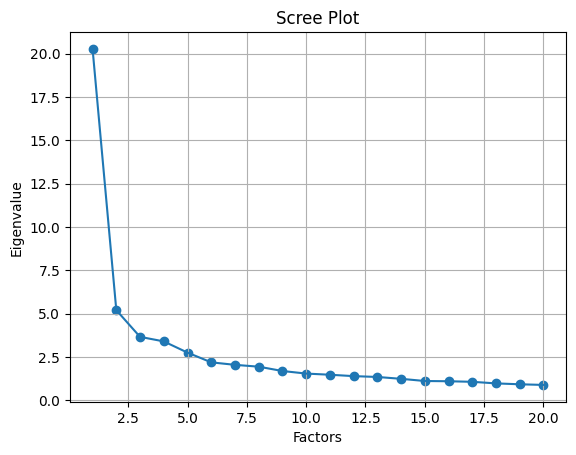
\includegraphics[width=\textwidth]{figures/scree.png}
    \caption{Scree plot indicated an elbow somewhere between 3 and 7 factors}
    \label{fig:model}
\end{figure}
\\
The first method was the Kaiser criterion, which states that factors with eigenvalues greater than 1 should be extracted.
This was first of all not feasable as it produced over 15 factors most of which with very low loadings and little domain relevance, with factors cross loading on multiple variables.
The second method was the scree plot, which is a visual method of determining the number of factors to extract, from this we determined that the elbow was somewhere between 3 and 7 factors (Figure 1). 
\\ 
Working first with seven factors we examined the loadings and domain relevance, we found that the factors had little domain relevace as well as low loadings. Strikingly Factors 5, 6, 7 only contained 3 practices each with loadings above 0.50. (Table 1).
\begin{landscape}
\small
\begin{longtable}{llllllllll}
\caption{Exploratory Factor Analysis - Highlighting loadings > 0.5} \label{tab:EFA} \\
\toprule
HPM Code & Factor 1 & Factor 2 & Factor 3 & Factor 4 & Factor 5 & Factor 6 & Factor 7 & Communality & Uniqueness \\
\midrule
\endfirsthead
\caption[]{Exploratory Factor Analysis - Highlighting loadings > 0.5} \\
\toprule
HPM Code & Factor 1 & Factor 2 & Factor 3 & Factor 4 & Factor 5 & Factor 6 & Factor 7 & Communality & Uniqueness \\
\midrule
\endhead
\midrule
\multicolumn{10}{r}{Continued on next page} \\
\midrule
\endfoot
\bottomrule
\endlastfoot
ENVRTX21 & \cellcolor{yellow}0.53 & 0.15 & -0.0 & 0.13 & -0.15 & 0.2 & -0.02 & 0.387124 & 0.612876 \\
ENVRTX37 & 0.14 & \cellcolor{yellow}0.6 & 0.06 & 0.08 & 0.03 & 0.06 & -0.06 & 0.401213 & 0.598787 \\
ENVRTX02 & \cellcolor{yellow}0.59 & 0.23 & 0.2 & 0.17 & 0.01 & -0.17 & -0.01 & 0.498194 & 0.501806 \\
ENVRTX22 & \cellcolor{yellow}0.6 & 0.14 & 0.23 & 0.1 & -0.15 & 0.13 & -0.07 & 0.490537 & 0.509463 \\
ENVRTX39 & \cellcolor{yellow}0.6 & 0.26 & 0.14 & 0.15 & 0.0 & 0.08 & -0.05 & 0.474416 & 0.525584 \\
ENVRTX23 & \cellcolor{yellow}0.65 & -0.07 & 0.05 & 0.16 & 0.08 & -0.15 & 0.2 & 0.526442 & 0.473558 \\
ENVRTX18 & \cellcolor{yellow}0.53 & 0.42 & 0.05 & 0.15 & 0.19 & 0.04 & -0.02 & 0.515498 & 0.484502 \\
ENVRTX13 & 0.46 & 0.29 & -0.05 & 0.13 & 0.19 & -0.07 & 0.09 & 0.364410 & 0.635590 \\
ENVRTX33 & 0.26 & \cellcolor{yellow}0.62 & 0.16 & 0.02 & -0.03 & 0.09 & 0.02 & 0.493124 & 0.506876 \\
ENVRTX03 & \cellcolor{yellow}0.6 & 0.12 & 0.16 & 0.25 & 0.09 & -0.0 & 0.04 & 0.475674 & 0.524326 \\
ENVRTX20 & \cellcolor{yellow}0.6 & 0.34 & 0.13 & 0.06 & -0.02 & 0.09 & 0.07 & 0.506159 & 0.493841 \\
ENVRTX38 & \cellcolor{yellow}0.6 & 0.36 & 0.15 & -0.0 & 0.07 & 0.01 & 0.15 & 0.546286 & 0.453714 \\
ENVRTX08 & \cellcolor{yellow}0.75 & -0.04 & 0.06 & 0.05 & 0.01 & -0.03 & 0.14 & 0.592730 & 0.407270 \\
ENVRTX05 & \cellcolor{yellow}0.75 & -0.02 & 0.12 & 0.09 & 0.04 & -0.19 & 0.16 & 0.652066 & 0.347934 \\
ENVRTX30 & 0.47 & 0.48 & 0.11 & 0.09 & 0.14 & 0.04 & -0.05 & 0.491478 & 0.508522 \\
ENVRTX24 & \cellcolor{yellow}0.66 & 0.22 & 0.31 & 0.07 & -0.02 & 0.07 & 0.13 & 0.613468 & 0.386532 \\
ENVRTX32 & 0.31 & \cellcolor{yellow}0.68 & 0.2 & 0.03 & -0.04 & 0.14 & -0.07 & 0.633967 & 0.366033 \\
ENVRTX34 & 0.32 & \cellcolor{yellow}0.55 & 0.11 & 0.03 & 0.08 & -0.0 & 0.1 & 0.428647 & 0.571353 \\
ENVRTX04 & \cellcolor{yellow}0.54 & 0.09 & 0.2 & 0.02 & 0.04 & 0.06 & 0.17 & 0.371735 & 0.628265 \\
ENVRTX29 & \cellcolor{yellow}0.55 & \cellcolor{yellow}0.57 & 0.15 & 0.11 & 0.16 & 0.04 & 0.03 & 0.694491 & 0.305509 \\
ENVRTX41 & 0.5 & 0.49 & 0.2 & -0.01 & 0.24 & 0.16 & -0.03 & 0.616388 & 0.383612 \\
ENVRTX40 & 0.46 & \cellcolor{yellow}0.54 & 0.23 & -0.01 & 0.07 & 0.21 & 0.04 & 0.609872 & 0.390128 \\
ENVRTX09 & \cellcolor{yellow}0.56 & 0.35 & 0.18 & 0.16 & 0.1 & 0.04 & -0.04 & 0.516182 & 0.483818 \\
ENVRTX17 & 0.29 & 0.5 & 0.31 & 0.11 & -0.11 & 0.13 & 0.15 & 0.490870 & 0.509130 \\
ENVRTX07 & 0.45 & 0.31 & 0.28 & 0.08 & -0.0 & 0.09 & 0.05 & 0.388896 & 0.611104 \\
ENVRTX11 & 0.47 & 0.43 & 0.18 & 0.1 & 0.14 & 0.2 & -0.07 & 0.513124 & 0.486876 \\
ENVRTX10 & 0.44 & 0.47 & 0.18 & 0.16 & 0.23 & 0.17 & -0.07 & 0.554014 & 0.445986 \\
ENVRTX01 & 0.47 & 0.13 & 0.26 & 0.1 & -0.06 & 0.16 & 0.19 & 0.377254 & 0.622746 \\
ENVRTX14 & \cellcolor{yellow}0.69 & 0.2 & 0.03 & 0.06 & 0.22 & -0.05 & 0.07 & 0.576579 & 0.423421 \\
ENVRTX15 & \cellcolor{yellow}0.64 & 0.25 & 0.01 & 0.07 & 0.17 & -0.16 & 0.14 & 0.546207 & 0.453793 \\
ENVRTX12 & 0.27 & 0.04 & 0.13 & 0.11 & 0.02 & 0.02 & \cellcolor{yellow}0.78 & 0.710872 & 0.289128 \\
ENVRTX31 & 0.29 & \cellcolor{yellow}0.51 & 0.19 & 0.18 & -0.1 & -0.06 & 0.37 & 0.560730 & 0.439270 \\
ENVRTX35 & 0.17 & \cellcolor{yellow}0.67 & 0.06 & 0.2 & 0.02 & -0.21 & 0.23 & 0.621047 & 0.378953 \\
ENVRTX36 & 0.1 & \cellcolor{yellow}0.69 & 0.22 & 0.19 & 0.08 & -0.08 & 0.13 & 0.597819 & 0.402181 \\
ENVRTX06 & 0.5 & 0.02 & 0.26 & -0.01 & 0.08 & -0.01 & 0.32 & 0.434361 & 0.565639 \\
EPRACX01 & 0.23 & 0.12 & 0.08 & 0.05 & 0.01 & 0.23 & \cellcolor{yellow}0.81 & 0.781392 & 0.218608 \\
EPRACX02 & 0.5 & 0.08 & 0.2 & -0.0 & 0.06 & 0.1 & \cellcolor{yellow}0.6 & 0.659780 & 0.340220 \\
EPRACX03 & \cellcolor{yellow}0.62 & 0.11 & 0.31 & 0.05 & -0.09 & 0.16 & 0.17 & 0.557559 & 0.442441 \\
EPRACX04 & \cellcolor{yellow}0.58 & 0.31 & 0.25 & 0.06 & -0.03 & 0.35 & 0.06 & 0.624820 & 0.375180 \\
EPRACX05 & \cellcolor{yellow}0.53 & 0.28 & 0.21 & 0.17 & -0.12 & 0.37 & 0.08 & 0.586183 & 0.413817 \\
EPRACX06 & \cellcolor{yellow}0.52 & 0.36 & 0.21 & 0.16 & 0.02 & 0.27 & -0.03 & 0.539612 & 0.460388 \\
EPERFX01 & 0.37 & 0.17 & \cellcolor{yellow}0.62 & 0.05 & 0.09 & -0.04 & 0.14 & 0.585140 & 0.414860 \\
EPERFX02 & 0.25 & 0.31 & \cellcolor{yellow}0.65 & 0.11 & 0.06 & 0.11 & -0.07 & 0.609480 & 0.390520 \\
EPERFX03 & 0.21 & 0.23 & \cellcolor{yellow}0.78 & 0.13 & 0.09 & -0.13 & -0.06 & 0.747198 & 0.252802 \\
EPERFX04 & 0.17 & 0.16 & \cellcolor{yellow}0.78 & 0.12 & 0.08 & -0.13 & -0.03 & 0.705412 & 0.294588 \\
EPERFX05 & 0.21 & 0.1 & \cellcolor{yellow}0.78 & 0.05 & 0.03 & 0.04 & 0.04 & 0.668555 & 0.331445 \\
EPERFX06 & 0.05 & 0.02 & \cellcolor{yellow}0.73 & 0.07 & -0.02 & 0.01 & 0.11 & 0.550325 & 0.449675 \\
EPERFX07 & 0.18 & 0.2 & \cellcolor{yellow}0.62 & 0.13 & 0.09 & 0.13 & 0.05 & 0.501326 & 0.498674 \\
EPERFX08 & 0.26 & 0.11 & \cellcolor{yellow}0.52 & 0.07 & 0.11 & 0.11 & 0.2 & 0.418796 & 0.581204 \\
EPERFX09 & 0.15 & 0.02 & \cellcolor{yellow}0.52 & 0.1 & -0.02 & -0.01 & 0.09 & 0.312394 & 0.687606 \\
LAYOUTN01 & 0.16 & -0.01 & 0.09 & \cellcolor{yellow}0.69 & 0.04 & -0.02 & 0.06 & 0.514815 & 0.485185 \\
LAYOUTN02 & 0.22 & 0.06 & 0.1 & \cellcolor{yellow}0.66 & -0.07 & 0.08 & -0.04 & 0.503373 & 0.496627 \\
LAYOUTN03 & 0.12 & 0.18 & 0.05 & \cellcolor{yellow}0.65 & -0.07 & 0.04 & 0.07 & 0.485319 & 0.514681 \\
LAYOUTN04 & 0.18 & 0.09 & 0.06 & \cellcolor{yellow}0.6 & 0.01 & 0.25 & 0.02 & 0.473988 & 0.526012 \\
JITDELN01 & 0.08 & 0.17 & 0.19 & 0.27 & 0.34 & 0.39 & 0.06 & 0.414861 & 0.585139 \\
JITDELN02 & 0.0 & 0.18 & 0.26 & 0.03 & 0.33 & 0.26 & -0.01 & 0.278420 & 0.721580 \\
JITDELN03 & -0.02 & 0.24 & 0.14 & 0.29 & 0.32 & 0.23 & -0.05 & 0.316878 & 0.683122 \\
KANBANN01 & -0.04 & 0.11 & 0.01 & -0.0 & 0.15 & \cellcolor{yellow}0.51 & 0.1 & 0.306588 & 0.693412 \\
KANBANN02 & 0.06 & -0.03 & -0.06 & 0.25 & 0.15 & \cellcolor{yellow}0.55 & 0.05 & 0.399152 & 0.600848 \\
KANBANN03 & 0.09 & -0.04 & -0.04 & 0.18 & 0.2 & \cellcolor{yellow}0.67 & 0.04 & 0.530976 & 0.469024 \\
LINKCN01 & 0.2 & -0.02 & 0.13 & 0.28 & \cellcolor{yellow}0.54 & 0.27 & -0.01 & 0.500219 & 0.499781 \\
LINKCN02 & 0.09 & -0.07 & 0.04 & 0.42 & 0.3 & 0.01 & 0.11 & 0.294498 & 0.705502 \\
LINKCN03 & -0.01 & -0.01 & 0.08 & 0.48 & 0.37 & -0.01 & -0.04 & 0.377006 & 0.622994 \\
LINKCN04 & 0.05 & 0.06 & 0.0 & 0.23 & \cellcolor{yellow}0.73 & 0.13 & 0.05 & 0.616880 & 0.383120 \\
LINKCN05 & 0.08 & 0.09 & 0.02 & 0.21 & \cellcolor{yellow}0.74 & 0.29 & 0.04 & 0.689089 & 0.310911 \\
SCHEDN01 & 0.05 & 0.07 & 0.04 & \cellcolor{yellow}0.59 & 0.15 & 0.1 & 0.08 & 0.395107 & 0.604893 \\
SCHEDN02 & 0.01 & 0.09 & 0.03 & \cellcolor{yellow}0.6 & 0.15 & 0.1 & 0.05 & 0.402938 & 0.597062 \\
SCHEDR03 & 0.07 & -0.21 & 0.09 & -0.05 & -0.14 & -0.15 & -0.0 & 0.103053 & 0.896947 \\
SETUPN01 & 0.17 & 0.05 & 0.02 & \cellcolor{yellow}0.53 & 0.12 & 0.0 & 0.01 & 0.324477 & 0.675523 \\
SETUPN02 & -0.04 & 0.18 & 0.16 & \cellcolor{yellow}0.57 & 0.04 & 0.05 & -0.04 & 0.390410 & 0.609590 \\
SETUPN03 & 0.17 & 0.21 & 0.15 & 0.46 & 0.35 & 0.02 & -0.09 & 0.435804 & 0.564196 \\
\end{longtable}

\end{landscape}
We then reduced the number of factors to 6 and then 5, and found that the factors had a higer domain relevant and had higher loadings, but still faced many cross loading issues especially with the Lean/JIT groups.
The domain relevance of these factors are also questionable as JIT was broken down into multiple factors with insufficient loadings to build a domain relevant factor.
Eventually we settled on 4 factors, which had high loadings and were domain relevant, revealing a domain relevant breakdown of the environmental practices while retaining the domain relevance of the Lean/JIT and enviromental performance groups.
3 factors also had high loadings and domain relevance, but as we had no reason to reject the breakdown in environmental practices suggested by the EFA we decided to continue with 4 factors. See Table 2, 3, 4 \& 5 below for a breakdown of our final bundles.
\begin{table}[htbp]
\centering
\caption{Environmental Practices 1 (General)}
\label{tab:your_label}
\begin{tabular}{lll}
\toprule
HPM Code & Description & Loadings \\
\midrule
ENVRTX08 & Decreasing Environmental Accident Impact & 0.851406 \\
ENVRTX05 & Pollution Prevention & 0.846418 \\
ENVRTX23 & Environmental Improvements for Scrap/Excess Materia... & 0.775964 \\
EPRACX02 & Internal Environmental Management Procedures & 0.671973 \\
ENVRTX14 & Industry-wide Code Compliance & 0.653831 \\
ENVRTX15 & Plant Compliance/Auditing Program & 0.629963 \\
EPRACX03 & Cleaner Production Technologies & 0.601676 \\
ENVRTX24 & Environmental Improvements for Equipment Dispositio... & 0.596048 \\
\bottomrule
\end{tabular}
\end{table} \\
\begin{table}[htbp]
\centering
\caption{Environmental Practices 2 (Suppliers)}
\label{tab:your_label}
\begin{tabular}{lll}
\toprule
HPM Code & Description & Loadings \\
\midrule
ENVRTX32 & Purchasing from M/WBE Suppliers & 0.823226 \\
ENVRTX33 & Formal M/WBE Supplier Purchase Program & 0.721714 \\
ENVRTX37 & Third Party Monitoring of Supplier Working Conditio... & 0.703129 \\
ENVRTX36 & Asking Suppliers for Living Wage & 0.662381 \\
ENVRTX29 & Encouraging Supplier Environmental Improvement & 0.641546 \\
ENVRTX40 & Co-development with Suppliers for Environmental Imp... & 0.620094 \\
ENVRTX34 & Ensuring No Sweatshop Labor in Supplier Plants & 0.605227 \\
ENVRTX35 & Ensuring Supplier Child Labor Law Compliance & 0.600539 \\
\bottomrule
\end{tabular}
\end{table} \\
\begin{table}[htbp]
\centering
\caption{JIT Practices}
\label{tab:your_label}
\begin{tabular}{lll}
\toprule
HPM Code & Description & Loadings \\
\midrule
LINKCN05 & Our customers are linked with us via JIT systems. & 0.623435 \\
SCHEDN02 & We usually complete our daily schedule as planned. & 0.621872 \\
SCHEDN01 & We usually meet the production schedule each day. & 0.619473 \\
LINKCN03 & We can adapt our production schedule to sudden prod... & 0.609956 \\
LINKCN04 & Our customers have a pull type link with us. & 0.594620 \\
LINKCN01 & Our customers receive just-in-time deliveries from ... & 0.592328 \\
LAYOUTN01 & Equipment Layout - Proximity & 0.591347 \\
LAYOUTN04 & Equipment Layout - JIT Production & 0.579354 \\
\bottomrule
\end{tabular}
\end{table} \\
\begin{table}[htbp]
\centering
\caption{Environmental Performance}
\label{tab:your_label}
\begin{tabular}{lll}
\toprule
HPM Code & Description & Loadings \\
\midrule
EPERFX06 & Releases to Water & 0.812363 \\
EPERFX04 & Water Consumption & 0.810310 \\
EPERFX05 & Emissions to Air & 0.804205 \\
EPERFX03 & Energy Consumption & 0.784988 \\
EPERFX02 & Raw Materials Consumption & 0.608603 \\
EPERFX07 & Solid Waste Generation & 0.607016 \\
EPERFX01 & Overall Environmental Performance & 0.584450 \\
EPERFX09 & Fines or Violations & 0.543801 \\
\bottomrule
\end{tabular}
\end{table} \\\\
\begin{table}[htbp]
\centering
\caption{Variance Explained by EFA}
\label{tab:your_label}
\begin{tabular}{llll}
\toprule
Factor & Eigenvalue & Variance Explained \% & Cumulative Variance Explained \% \\
\midrule
Factor 1 & 20.274239 & 26.770974 & 26.770974 \\
Factor 2 & 5.197752 & 6.296780 & 33.067754 \\
Factor 3 & 3.654683 & 4.362066 & 37.429821 \\
Factor 4 & 3.393518 & 3.945660 & 41.375481 \\
Factor 5 & 2.746089 & 3.003128 & 44.378609 \\
Factor 6 & 2.184200 & 2.426975 & 46.805584 \\
Factor 7 & 2.040140 & 2.098922 & 48.904506 \\
\bottomrule
\end{tabular}
\end{table} \\\\
One remaining point on the EFA process recommended by \citep{beaversPracticalConsiderationsUsing2013} is to check the amount of variance explained by the factors.
We found that the 4 factor model explained ~41\% of the variance in the data, while the 7 factor model explained ~49\% of the variance in the data.
Due to the lack of interpretability of the 7 factor model and above models we decided to continue with the 4 factor model. (Table 6)
\\
Although \citep{furlanComplementarityLeanManufacturing2011} used a CFA to identify the factors, we have used an EFA to identify smaller bundles and validate theoretical assumptions. We also performed a CFA based on the relevant HPM round 4 scales. The results of the CFA analysis are included in the appendix.
\subsection*{Complimentarity Analysis}
The first step in the complimentarity analysis as demonstrated by \citep{furlanComplementarityLeanManufacturing2011} was to create a dummy variable for each bundle based on the factors.
Dummy variables were created for each bundle, with the dummy variable being 1 if the firm scored above the median on all practices in the bundle, and 0 otherwise.
From these 4 categories were constructed based on the combinations of bundles, these categories are:
\begin{itemize}
    \item High JIT \& Environmental
    \item Low JIT \& Environmental
    \item Mainly Environmental
    \item Mainly JIT
\end{itemize}
See table 7 below for a breakdown of the categories.
\begin{table}[htbp]
    \centering
    \caption{Frequency of Adoption and Environmental Performance}
    \label{tab:your_label}
    \begin{tabular}{lrll}
\toprule
Category & Frequency & Percentage & Mean of Performance \\
\midrule
High JIT \& Environmental & 57 & 32.57 & 3.91 \\
Mainly Environmental & 38 & 21.71 & 3.78 \\
Mainly JIT & 40 & 22.86 & 3.58 \\
Low JIT \& Environmental & 40 & 22.86 & 3.28 \\
\bottomrule
\end{tabular}

    \end{table}
    
The next step was to conduct a Tukey HSD test to determine if there was a significant difference between the mean environmental performance of the four groups.
The results of the Tukey HSD test will be discussed in the results section.
\subsection*{Regression Analysis}
The final step in the analysis was to conduct a regression analysis to determine if there was a significant moderating effect of JIT on the relationship between environmental practices and environmental performance.
The regression analysis was conducted using the \texttt{statsmodels} package for Python \citep{seaboldStatsmodelsEconometricStatistical2010}.

\section{Results}
adf ba 
\section{Discussion}
TBA
\bibliographystyle{plainnat} % This style is compatible with natbib and author-year
\bibliography{\jobname}
\section*{Appendix}
\begin{table}[htbp]
\centering
\caption{Multiple Comparison of Means - Tukey HSD, FWER=0.05}
\label{tab:your_label}
\begin{tabular}{llrrrrr}
\toprule
group1 & group2 & p-adj & lower & upper & reject \\
\midrule
High JIT \& Environmental & Low JIT \& Environmental & 0.00 & -0.85 & -0.28 & True \\
High JIT \& Environmental & Mainly Environmental & 0.69 & -0.43 & 0.18 & False \\
High JIT \& Environmental & Mainly JIT & 0.00 & -0.65 & -0.14 & True \\
Low JIT \& Environmental & Mainly Environmental & 0.01 & 0.09 & 0.79 & True \\
Low JIT \& Environmental & Mainly JIT & 0.45 & -0.13 & 0.48 & False \\
Mainly Environmental & Mainly JIT & 0.15 & -0.59 & 0.06 & False \\
\bottomrule
\end{tabular}\end{table}
\begin{table}[htbp]
    \centering
    \caption{Emissions to Air - Regression Results (Based on CFA Bundles)}
    \label{tab:regression}
    \begin{tabular}{lccccccc}
\toprule
Coefficient & Coef. & Std.Err. & t & P>|t| & [0.025 & 0.975] & Sig. \\
\midrule
Intercept & -0.86 & 1.81 & -0.48 & 0.63 & -4.43 & 2.70 &  \\
Env\_Score & 1.26 & 0.52 & 2.42 & 0.02 & 0.23 & 2.28 & ** \\
JIT\_Score & 0.83 & 0.53 & 1.58 & 0.12 & -0.21 & 1.87 &  \\
JIT\_Env\_Interaction & -0.22 & 0.15 & -1.48 & 0.14 & -0.51 & 0.07 &  \\
ACCTGX51 & -0.00 & 0.00 & -0.09 & 0.93 & -0.00 & 0.00 &  \\
\bottomrule
\end{tabular}

    \end{table}
    
\begin{table}[htbp]
    \centering
    \caption{Solid Waste Generation - Regression Results (Based on CFA Bundles)}
    \label{tab:regression}
    \begin{tabular}{lccccccc}
\toprule
Coefficient & Coef. & Std.Err. & t & P>|t| & [0.025 & 0.975] & Sig. \\
\midrule
Intercept & 1.50 & 1.58 & 0.95 & 0.35 & -1.63 & 4.62 &  \\
Env\_Score & 0.46 & 0.45 & 1.02 & 0.31 & -0.43 & 1.36 &  \\
JIT\_Score & 0.27 & 0.46 & 0.58 & 0.56 & -0.64 & 1.18 &  \\
JIT\_Env\_Interaction & -0.02 & 0.13 & -0.19 & 0.85 & -0.28 & 0.23 &  \\
ACCTGX51 & 0.00 & 0.00 & 1.41 & 0.16 & -0.00 & 0.00 &  \\
\bottomrule
\end{tabular}

    \end{table}
    
\begin{landscape}
\small
\begin{longtable}{l@{\hspace{6pt}}l@{\hspace{6pt}}p{11cm}@{\hspace{6pt}}l@{\hspace{6pt}}l@{\hspace{6pt}}l}
\caption{Confirmatory Factor Analysis} \label{tab:your_label} \\
\toprule
Bundle & HPM Code & Item Description & Loading & SE & t-value \\
\midrule
\endfirsthead
\caption[]{Confirmatory Factor Analysis} \\
\toprule
Bundle & HPM Code & Item Description & Loading & SE & t-value \\
\midrule
\endhead
\midrule
\multicolumn{6}{r}{Continued on next page} \\
\midrule
\endfoot
\bottomrule
\endlastfoot
Environmental Practices & ENVRTX21 & Environmentally preferable packaging for the products that you produce (recycled content, less volume, reusable packaging) & 0.63*** & 0.06 & 11.11 \\
 & ENVRTX37 & Using a third party to monitor working conditions at supplier facilities & 0.8*** & 0.08 & 9.75 \\
 & ENVRTX02 & Water efficiency & 0.88*** & 0.07 & 12.97 \\
 & ENVRTX22 & Substituting environmental preferable direct materials or supplies for harmful or non-renewable ones & 0.69*** & 0.06 & 11.44 \\
 & ENVRTX39 & Providing design specification to suppliers in line with environmental requirements (e.g. green purchasing, black list of raw materials) & 1.06*** & 0.08 & 13.5 \\
 & ENVRTX23 & Environmental improvements in the disposition of your organization’s scrap or excess material (re-use, recycling, etc.) & 0.58*** & 0.05 & 10.82 \\
 & ENVRTX18 & Working with customers to help them achieve environmental objectives & 1.12*** & 0.08 & 14.25 \\
 & ENVRTX13 & Complying with a customer’s supplier code of conduct & 0.91*** & 0.08 & 11.8 \\
 & ENVRTX33 & Starting or maintaining a formal M/WBE supplier purchase program & 1.0*** & 0.08 & 11.79 \\
 & ENVRTX03 & Reducing waste in internal processes (e.g., improving yield or efficiency) & 0.61*** & 0.05 & 11.79 \\
 & ENVRTX20 & Life-cycle analysis of the “cradle to grave” environmental impact of materials/products & 1.19*** & 0.08 & 14.62 \\
 & ENVRTX38 & Incorporating environmental considerations in evaluating and selecting suppliers & 1.16*** & 0.07 & 15.53 \\
 & ENVRTX08 & Decreasing the likelihood or impact of an environmental accident & 0.67*** & 0.05 & 12.3 \\
 & ENVRTX05 & Pollution prevention (eliminating emissions or waste) & 0.72*** & 0.06 & 12.89 \\
 & ENVRTX30 & Giving preference to materials with third party certifications, such as Green Seal, FSC or Energy Star & 1.02*** & 0.08 & 13.2 \\
 & ENVRTX24 & Environmental improvements in the disposition of your organization’s equipment & 0.97*** & 0.06 & 15.36 \\
 & ENVRTX32 & Purchasing from minority- or women-owned business enterprise (M/WBE) suppliers & 0.98*** & 0.08 & 12.96 \\
 & ENVRTX34 & Visiting suppliers’ plants or ensuring that they are not using sweatshop labor & 1.07*** & 0.09 & 12.5 \\
 & ENVRTX04 & Improving the workforce environment (e.g., indoor air quality) & 0.57*** & 0.05 & 11.27 \\
 & ENVRTX29 & Encouraging suppliers to improve the environmental performance of their processes & 1.28*** & 0.08 & 16.88 \\
 & ENVRTX41 & Involvement of suppliers in the re-design of internal processes (e.g. remanufacturing, reduction of by-products) & 1.02*** & 0.07 & 14.73 \\
 & ENVRTX40 & Co-development with suppliers to reduce the environmental impact of the product (e.g. eco-design, green packaging, recyclability) & 1.09*** & 0.07 & 15.24 \\
 & ENVRTX09 & Reduction/avoidance of land consumption & 1.13*** & 0.09 & 13.24 \\
 & ENVRTX17 & Carbon tracking/carbon footprint calculation of supply chain & 1.11*** & 0.09 & 12.68 \\
 & ENVRTX07 & Remediation projects, such as cleanup or restoration from past practices & 1.18*** & 0.09 & 12.57 \\
 & ENVRTX11 & Improvements in outbound transportation, such as fuel efficiency or load matching & 1.12*** & 0.08 & 14.1 \\
 & ENVRTX10 & Improvements in inbound transportation, such as fuel efficiency or load matching & 1.1*** & 0.08 & 14.38 \\
 & ENVRTX01 & Energy efficiency or renewable energy & 0.77*** & 0.07 & 11.55 \\
 & ENVRTX14 & Complying with an industry-wide code of conduct & 0.87*** & 0.06 & 14.21 \\
 & ENVRTX15 & Other compliance or auditing program focused on your plant (not on your suppliers) & 0.88*** & 0.06 & 13.72 \\
 & ENVRTX12 & Seeking or maintaining ISO14001 certification & 0.85*** & 0.09 & 9.73 \\
 & ENVRTX31 & Requesting that your suppliers sign a code of environmental conduct & 1.16*** & 0.09 & 12.72 \\
 & ENVRTX35 & Ensuring that suppliers comply with child labor laws & 1.12*** & 0.1 & 11.7 \\
 & ENVRTX36 & Asking suppliers to pay a “living wage” & 1.04*** & 0.09 & 11.17 \\
 & ENVRTX06 & Pollution control (scrubbing, waste treatment) & 0.76*** & 0.07 & 11.27 \\
 & EPRACX01 & Implementation of a certified environmental management system, such as ISO 14000. & 0.96*** & 0.09 & 10.3 \\
 & EPRACX02 & Implementation of internal environmental management procedures (e.g. environmental training program, internal environmental audit, newsletter). & 0.96*** & 0.08 & 12.34 \\
 & EPRACX03 & Use of cleaner technologies in the production process (e.g. abatement equipment) to reduce pollution emissions and/or resource use. & 0.98*** & 0.07 & 14.2 \\
 & EPRACX04 & Environment-friendly product design. & 1.21*** & 0.08 & 15.58 \\
 & EPRACX05 & Environmental improvement of packaging. & 1.0*** & 0.07 & 14.74 \\
 & EPRACX06 & Use of environment-friendly raw materials. & 0.99*** & 0.07 & 14.6 \\
JIT Practices & LAYOUTN01 & We have laid out the shop floor so that processes and machines are in close proximity to each other. & 0.71*** & 0.06 & 11.66 \\
 & LAYOUTN02 & The layout of our shop floor facilitates low inventories and fast throughput. & 0.79*** & 0.07 & 12.04 \\
 & LAYOUTN03 & Our processes are located close together, so that material handling and part storage are minimized. & 0.88*** & 0.07 & 11.87 \\
 & LAYOUTN04 & We have located our machines to support JIT production flow. & 1.03*** & 0.08 & 13.77 \\
 & JITDELN01 & Our suppliers deliver to us on a just-in-time basis. & 1.09*** & 0.09 & 12.74 \\
 & JITDELN02 & We receive daily shipments from most suppliers. & 0.8*** & 0.09 & 9.13 \\
 & JITDELN03 & Our suppliers are linked with us by a pull system. & 1.1*** & 0.09 & 12.2 \\
 & KANBANN01 & Suppliers fill our kanban containers, rather than filling purchase orders. & 0.73*** & 0.09 & 8.39 \\
 & KANBANN02 & We use a kanban pull system for production control. & 1.05*** & 0.09 & 11.34 \\
 & KANBANN03 & We use kanban squares, containers or signals for production control. & 1.08*** & 0.09 & 11.56 \\
 & LINKCN01 & Our customers receive just-in-time deliveries from us. & 1.04*** & 0.08 & 12.82 \\
 & LINKCN02 & We always deliver on time to our customers. & 0.71*** & 0.06 & 10.97 \\
 & LINKCN03 & We can adapt our production schedule to sudden production stoppages by our customers. & 0.77*** & 0.07 & 11.39 \\
 & LINKCN04 & Our customers have a pull type link with us. & 1.18*** & 0.09 & 12.66 \\
 & LINKCN05 & Our customers are linked with us via JIT systems. & 1.24*** & 0.09 & 13.44 \\
 & SCHEDN01 & We usually meet the production schedule each day. & 0.75*** & 0.06 & 12.46 \\
 & SCHEDN02 & We usually complete our daily schedule as planned. & 0.68*** & 0.05 & 12.59 \\
 & SETUPN01 & We are aggressively working to lower setup times in our plant. & 0.76*** & 0.07 & 10.88 \\
 & SETUPN02 & We have low setup times of equipment in our plant. & 0.81*** & 0.07 & 11.53 \\
 & SETUPN03 & Our workers practice setups, in order to reduce the time required. & 1.04*** & 0.09 & 11.84 \\
Environmental Performance & EPERFX01 & Overall environmental performance. & 0.83*** & 0.06 & 14.96 \\
 & EPERFX02 & Raw materials consumption. & 0.77*** & 0.05 & 14.78 \\
 & EPERFX03 & Energy consumption. & 0.96*** & 0.06 & 16.74 \\
 & EPERFX04 & Water consumption. & 0.94*** & 0.06 & 17.02 \\
 & EPERFX05 & Emissions to air. & 0.89*** & 0.06 & 15.69 \\
 & EPERFX06 & Releases to water. & 0.81*** & 0.06 & 14.38 \\
 & EPERFX07 & Solid waste generation (e.g. landfill capacity consumed). & 0.7*** & 0.05 & 13.53 \\
 & EPERFX08 & Waste recovery (e.g. recycling). & 0.59*** & 0.05 & 11.7 \\
 & EPERFX09 & Fines or other violations of environmental rules/regulations. & 0.84*** & 0.07 & 11.57 \\
\end{longtable}

\end{landscape}

\end{document}